\documentclass[tikz,border=4pt]{standalone}
\usetikzlibrary{arrows.meta,positioning,calc,fit}
\begin{document}
% Canvas 20 x ~10.5 cm (same aspect as the earlier diagram).
% Fixes vs the earlier version: the decoder is NOT a plain Conv2DTranspose stack (it outputs the last observed
% depth frame + a learned change, with a skip connection from the encoder), and the capsule head does NOT end in a
% 4-way softmax (it outputs one capsule length per class, trained with the CapsNet margin loss; argmax = class).
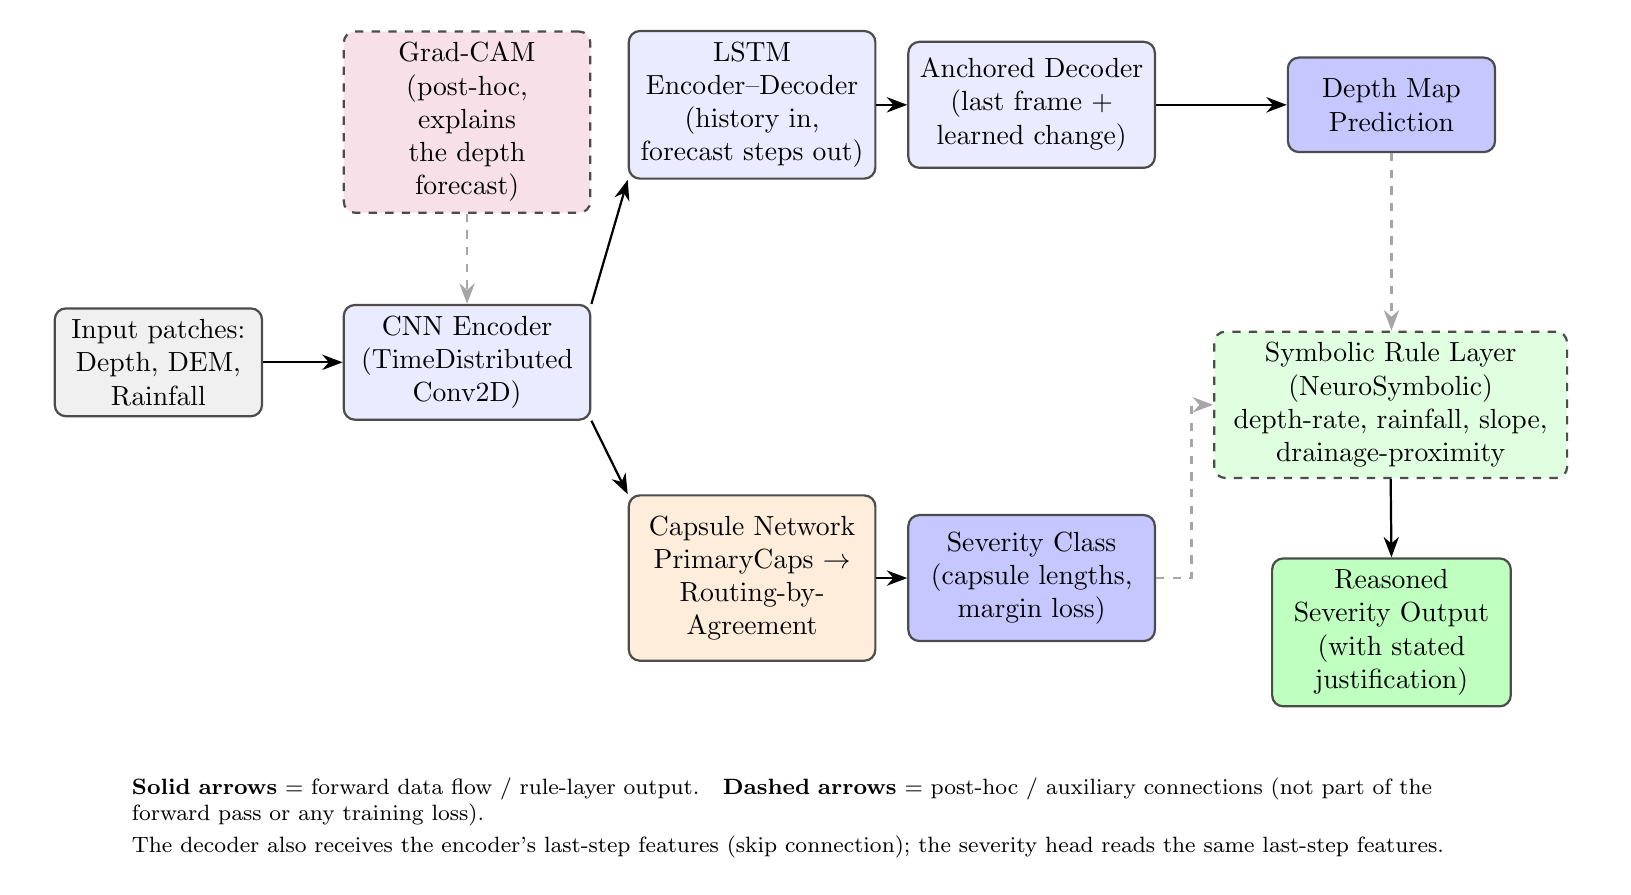
\begin{tikzpicture}[
    x=1cm, y=1cm, font=\normalsize,
    box/.style={draw=black!70, rounded corners=4pt, thick, align=center, inner sep=4pt, minimum height=1.25cm},
    solid/.style={-{Stealth[length=2.6mm]}, thick, black},
    dashd/.style={-{Stealth[length=2.6mm]}, thick, dashed, black!35},
]
% ---- nodes (centres in cm; y grows upward) ----
\node[box, fill=black!6,   text width=2.35cm, minimum height=1.20cm] (inp)  at (1.66,5.90)  {Input patches: Depth, DEM, Rainfall};
\node[box, fill=blue!8,    text width=2.85cm, minimum height=1.30cm] (enc)  at (5.58,5.90)  {CNN Encoder \\ (\mbox{TimeDistributed} \\ Conv2D)};
\node[box, fill=purple!12, dashed, text width=2.85cm, minimum height=1.60cm] (gc) at (5.58,8.95) {Grad-CAM \\ (post-hoc, explains \\ the depth forecast)};
\node[box, fill=blue!8,    text width=2.85cm, minimum height=1.60cm] (lstm) at (9.20,9.17)  {LSTM \\ \mbox{Encoder--Decoder} \\ (history in, \\ forecast steps out)};
\node[box, fill=blue!8,    text width=2.85cm, minimum height=1.60cm] (dec)  at (12.75,9.17) {Anchored Decoder \\ (last frame + \\ learned change)};
\node[box, fill=blue!22,   text width=2.35cm, minimum height=1.20cm] (depth) at (17.32,9.17) {Depth Map Prediction};
\node[box, fill=orange!14, text width=2.85cm, minimum height=2.10cm] (caps) at (9.20,3.16)  {Capsule Network \\ PrimaryCaps $\rightarrow$ \\ Routing-by- \\ Agreement};
\node[box, fill=blue!22,   text width=2.85cm, minimum height=1.60cm] (sev)  at (12.75,3.16) {Severity Class \\ (capsule lengths, \\ margin loss)};
\node[box, fill=green!12,  dashed, text width=4.20cm, minimum height=1.45cm] (sym) at (17.31,5.36) {Symbolic Rule Layer (NeuroSymbolic) \\ depth-rate, rainfall, slope, \\ drainage-proximity};
\node[box, fill=green!25,  text width=2.75cm, minimum height=1.60cm] (out)  at (17.32,2.47) {Reasoned Severity Output \\ (with stated justification)};

% ---- solid data flow ----
\draw[solid] (inp.east) -- (enc.west);
\draw[solid] (enc.north east) -- (lstm.south west);
\draw[solid] (enc.south east) -- (caps.north west);
\draw[solid] (lstm.east) -- (dec.west);
\draw[solid] (dec.east) -- (depth.west);
\draw[solid] (caps.east) -- (sev.west);
\draw[solid] (sym.south) -- (out.north);
% ---- dashed (post-hoc / auxiliary) ----
\draw[dashd] (gc.south) -- (enc.north);
\draw[dashd] (depth.south) -- (depth |- sym.north);
\draw[dashd] (sev.east) -- ++(0.45,0) |- (sym.west);

% ---- legend ----
\node[align=left, font=\footnotesize, text width=17.6cm, anchor=north west] at (1.2,0.75)
  {\hyphenpenalty=10000 \textbf{Solid arrows} = forward data flow / rule-layer output.\quad \textbf{Dashed arrows} = post-hoc / auxiliary connections (not part of the forward pass or any training loss).\\[2pt]
   The decoder also receives the encoder's last-step features (skip connection); the severity head reads the same last-step features.};
\useasboundingbox (0,-0.35) rectangle (20,10.15);
\end{tikzpicture}
\end{document}
